\chapter{Technique Indicators}
\label{append:technical_indicator}

Technical analysis is one of the oldest security analysis methodology. A qualified technician predicts the direction of prices and makes buy or sell decision under the help of all kinds of charts and indicators.\\


This study also covers some indicators, the details of which can be find below.


\section{Moving Average (MA)\cite{kahn2006technical}}
A \textit{moving average} is the average price of a stock or market over a given period. MA helps neglect fluctuations and catch the main trend. Two basic type of MAs are used in this study.

\subsection{Simple Moving Average (SMA)}
SMA is the simplest MA. Assume that the price at time t is $ p_t $ where $t=1,2,3,\ldots$, $n$ is the given period, then the SMA at time $ t $ with $ n $ periods is
\begin{equation}
SMA(t, n)=\frac{\sum_{i=0}^{n-1}p_{t-i}}{n}
\end{equation}

\subsection{Exponential Moving Average (EMA)}  
SMA pays equal attention to every historical price. But, intuitively, the closer the stock price, the more significant it is in forecasting future price. To solve this problem, people developed EMA, which gives later prices higher weights than prior ones. Let $ K =\frac{2}{n+1} $, then EMA is 
\begin{equation}
EMA(t) = K\times p_t+(1-K) \times EMA(t-1)
\end{equation}

A comparison between EMA and SMA can be find in figure~\ref{fg:smaema}.
\begin{figure}[h]
	\centering
	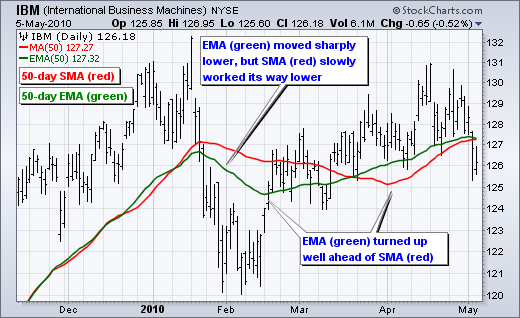
\includegraphics[width=0.8\textwidth]{EmaSma}
	\caption{Comparison between EMA and SMA\cite{9_sma_ema}}
	\label{fg:smaema}
\end{figure}

\section{Rate of Change (ROC)}
ROC is a simple way of measure the speed at which the price changes\cite{pring2002technical}. ROC can be calculated by
\begin{equation}
	ROC(n) = 100\times\frac{p_t}{p_{t-n}}
\end{equation}


\section{Relative Strength Index (RSI)}
RSI which was developed by Wells Wilder, measures change and speed of stock price relative strength\cite{pring2002technical}. The formula for RSI is
\begin{equation}
RSI = 100 - \frac{100}{1 + RS}
\end{equation}
where RS is
\begin{gather*}
RS=\frac{\text{Average Gain}}{\text{Average Loss}}\\
\end{gather*}
RSI value fluctuates in a constant range between 0 and 100. Usually, overbought and oversold lines are drawn at the 70 and 30 level\cite{pring2002technical}

\section{Moving Average Convergence Divergence (MACD)}
MACD measures the distance between two EMA lines (with different periods), and was developed by Gerald Appel\cite{kahn2006technical}. MACD can be calculted through,
\begin{equation}
MACD(m,n)=EMA(m)-EMA(n)
\end{equation}
Usually $ m < n $. The most widely used parameter for MACD is using 12-day EMA minus 26-day EMA\cite{kahn2006technical}.